\chapter{Background Theory}
\section{Magnetism}
Where charge ($\vec{E}$-field) has an elementary source unit of a point charge (or monopole) which may be positively or negatively charged. Conversely the elementary source unit of magnetism ($\vec{B}$-field) is the \index{magnetic dipole}{magnetic dipole}. 


\begin{figure}[H]
    \begin{center}
        \begin{tikzpicture}[thick, scale=1.4]
  \foreach \i [evaluate={\angle=(\i-1)*360/\NE;}] in {1,...,\NE}{
    \draw[EFieldLineArrow={0.45}] (\angle:\R) -- (0,0);
  }
  % \foreach \i [evaluate={\r=0.9*\R/\i;}] in {1,...,\NV}{
    % \draw[EcolEP] (0,0) circle (\r);
  % }
  \draw[charge-] (0,0) circle (7pt) node[black,scale=0.8] {$-q$};

  \node at (0,-1.35*\R) {$\vec{\nabla}\cdot{{\color{veccol}\vec{E}}} \propto \rho $};
\end{tikzpicture}

        \hspace{2cm}
        % ZERO
\begin{tikzpicture}[thick, scale=1.4]
  \def\ang{60}
  % \fill[myblue] (0,0) circle (\r);
  \foreach \x/\y in {-1/0,-1/1,0/1,1/1,1/0,-1/-1,0/-1,1/-1}{
    \draw[vector] (\x*0.5*\R,\y*0.5*\R) ++ (\ang-180:\R/2) --++ (\ang:\R);
  }

  \draw[charged] (0,0) circle (7pt) node[black,scale=0.8] {$\mu$};
  \node at (0,-1.35*\R) {$\vec{\nabla}\cdot{{\color{veccol}\vec{B}}} = 0$};
\end{tikzpicture}


        % \includegraphics[width=0.95\textwidth]{figures/}
    \end{center}
    \caption{Schematic of electric monopole and magnetic dipole with associated field lines and relevant Maxwell equation.}\label{fig:}
\end{figure}

\index{magnetic monopole}{Magnetic monopole}s have never been observed; their existence would also violate Gauss' law ($\vec{\nabla} \cdot \vec{B} = 0 $) \cite{Jackson1998-er}. 

\subsection{Magnetic Dipole}
Classically, the magnetic dipole is though of as a loop carrying an
electric current ($I$). 

The resultant \index{magnetic dipole moment}{magnetic dipole moment}, $\vec{\mu}$, is defined as the vector at a normal to the  
plane of the current loop, 
\begin{equation}
    \vec{\mu} = IS \vec{n}
    \label{eq:dipole_moment}
\end{equation}
where $I$ is the current in, and $S$ the surface area enclosed by, the loop. 

\begin{wrapfigure}{l}{0.4\textwidth}%
    \centering%
    % 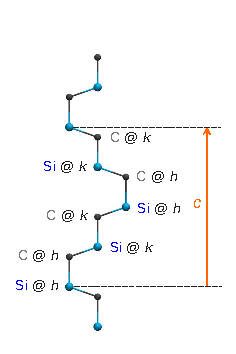
\includegraphics[width=0.38\textwidth]{figures/SiC-non-equiv-sites.pdf}%
        % B FIELD through current loop
\begin{tikzpicture}[scale=1.2, thick]
  \def\Rx{1.45}
  \def\Ry{0.43}
  \def\h{0.5}
  \def\H{3}
  \def\L{4}
  \def\NB{5}
  \def\ang{36}
  \coordinate (O) at (0,0);
  \coordinate (N) at (0,0.24*\H);
  \coordinate (M) at (0,0.45*\H);
  \coordinate (B) at (\ang:\H);
  
  % MAGNETIC FIELD
  \draw (-\Rx,0) arc (180:0:{\Rx} and {\Ry});
  \begin{scope}
    \clip ({-0.5*\L*cos(\ang)},-0.4*\H) rectangle ++({\L*cos(\ang)},\H);
    %\foreach \i [evaluate={\y=(\i-0.5)*\H/(\NB-0.5)/2;
    %                       \yl=-\H/2+(\i-0.5)*\H/(\NB-0.5)/2;}] in {1,...,\NB}{
    %  %\draw[BFieldLine,thin] (0,\y)++(\ang-180:0.5*\L) --++ (\ang:\L);
    %  %\draw[BFieldLine,thin] (0,-\y)++(\ang-180:0.5*\L) --++ (\ang:\L);
    %  \draw[BFieldLine,thin] (-\H/2,\y) -- ({-\H/2+(\H/2-\y)*cos(\ang)},\H/2);
    %  \draw[BFieldLine,thin] (-\H/2,-\y) -- ({-\H/2+(\H/2+\y)*cos(\ang)},+\H/2);
    %  \draw[BFieldLine,thin] ({\H/2-(\H/2+\yl)*cos(\ang)},-\H/2) -- (\H/2,\yl);
    %  \draw[BFieldLine,thin] ({\H/2-(\H/2-\yl)*cos(\ang)},-\H/2) -- (\H/2,-\yl);
    %}
    % \foreach \i [evaluate={\x=-0.31*\H+(\i-1)*0.62*\H/(\NB-1);
    %                        \y=-cot(\ang)*\x;
    %                        \a=0.50+0.017*\i}] in {1,...,\NB}{ %0.58-0.02*(\i-\NB/2-1)^2
    %   \draw[BFieldLine=\a] (\x,\y)++(\ang-180:\H) --++ (\ang:2*\H);
      %\fill[red] (\x,\y) circle (0.05);
    % }
  \end{scope}
  % \node[Bcol] at (\H/2,0.49*\H) {$\vb{B}$};
  
  % CIRCUIT
  \draw[white,very thick]
        (-\Rx,0) arc (-180:0:{\Rx} and {\Ry});
  \draw (-\Rx,0) arc (-180:0:{\Rx} and {\Ry});
  %\draw[white,very thick] (0,0) ellipse ({\R} and {0.3*\R});
  %\draw (0,0) ellipse ({\R} and {0.3*\R});
  %\draw (0,0) ellipse ({\R} and {0.3*\R});
  \draw[mu vector] (0,0) -- (M) node[above=-1, left=0] {$\vb*{\mu}$};
  \draw[vector] (0,0) -- (N) node[below=0,left=0] {$\vu{n}$};
  % \draw pic[->,"\small$\;\theta$",draw=black,angle radius=14,angle eccentricity=1.4]
    % {angle = B--O--N};
  \draw[white,very thick]
    (-150:{1.1*\Rx} and {1.16*\Ry}) arc (-150:-80:{1.1*\Rx} and {1.16*\Ry});
  \draw[current]
    (-135:{1.1*\Rx} and {1.16*\Ry}) arc (-135:-90:{1.1*\Rx} and {1.16*\Ry})
    node[midway,right=2,below] {$I$};
  
\end{tikzpicture}


  \caption{Schematic of current loop and induced magnetic moment.}%
\end{wrapfigure}%


The \index{magnetic dipole}{magnetic dipole} induces a magnetic field $\vec{B}$, which for points a large distance from the dipole may be calculated as \cite{Griffiths2012-pt}:
\begin{equation}
    \vec{B} = \frac{\mu_0}{4\pi} \frac{1}{r^3} \left[\frac{3(\vec{\mu} \cdot \vec{r}) \cdot \vec{r}}{r^2} - \vec{\mu}\right]
    \label{eq:}
\end{equation}

The symmetry of the field enables us to consider the direction of the dipole as aligned to the $z$-axis. Then, defining $x,y$ as usual by $r \cos\theta$ and $r \sin\theta$ respectively. We may decompose the \index{magnetic field}{magnetic field} in two separate components, parallel ($B_z$) and perpendicular ($B_x, B_y$): 
$$B_\parallel =\frac{\mu_0}{r^3}(3\cos^2 \theta - 1), \quad B_\perp = \frac{3\mu_0}{r^3}\cos\theta\sin\theta.$$
Where we use the Pythagorean principle to determine the overall magnitude $B = |\vec{B}|$ as
$$B = \sqrt{B_\parallel^2 + B_\perp^2}.$$

\subsection{Gyromagnetic Ratio}
\subsubsection{Classical Derivation}
The current in equation \ref{eq:dipole_moment} is proportional to the angular momentum of the charge. That is, the dipole moment is always associated with an angular momentum $\vec{G} = \vec{r} \times \vec{p}$ with $\vec{r}$ the radius and $\vec{p}$ the momentum. 

Dividing the magnetic dipole moment by the angular momentum we find the \textbf{gyromagnetic ratio}. 
\begin{equation}
    \gamma = \frac{\vec{\mu}}{\vec{G}}.
    \label{eq:gyromagnetic_ratio}
\end{equation}

Without loss of generality we may consider the most simple case which is where the magnetic dipole moment is parallel (or anti-parallel) to the angular momentum. Then we may consider the absolute values for the dipole moment and the angular momentum: 
\begin{equation}
    \mu = IS, \quad I = 
    % \underbrace{\frac{q}{2\pi R}}_{\rho \text{ (charge density)}}v,
    \frac{qv}{2\pi R},
    \quad S = \pi R^2 
    % \label{eq:}
\end{equation}
We substitute $I$ and $S$ to find 
\begin{equation}
    \mu = \frac{qvR}{2} 
    % \label{eq:}
\end{equation}
% which we substitute into our equation for the gyromagnetic ratio 
% \begin{equation}
%     \gamma = \frac{\frac{qvR}{2}}{\vec{G}}. 
%     \label{eq:789}
% \end{equation}
and further, we equate the angular momentum vector, using the model of a planar loop to 
\begin{equation}
   G= m_q v R 
    % \label{eq:}
\end{equation}
leaving 
\begin{equation}
    \gamma = \frac{q}{2m_q } . 
    % \label{eq:}
\end{equation}

We finally consider that we may represent the, currently unknown, charge and mass as a sum of electron charges and masses. 
\begin{equation}
    \gamma = \frac{q}{2m_q } = \frac{\cancel{N}e}{2\cancel{N} m_e} \implies \gamma = \frac{e}{2 m_e}
    \label{eq:gyromagnetic_ratio}
\end{equation}

We therefore find that the gyromagnetic ratio of the electron depends only on fundamental constants \cite{bromley2000quantum}.

%pg 329 
% https://www.google.co.uk/books/edition/_/7qCMUfwoQcAC?hl=en&gbpv=1&bsq=walter%20greiner%20theoretical%20physics



\subsubsection{Extending to Quantum Mechanics}
Since the gyromagnetic ratio was calculated considering the motion of dipole in a loop, we may extend this to an electron in an orbit.

\begin{wrapfigure}{r}{0.5\textwidth}%
	% \centering%
	\begin{center}
		% 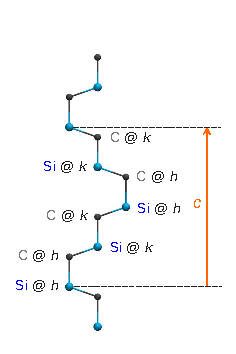
\includegraphics[width=0.38\textwidth]{figures/SiC-non-equiv-sites.pdf}%
		% MAGNETIC MOMENT ATOM
\begin{tikzpicture}[thick, scale=1.5]
  \def\rn{0.3}
  \def\re{0.15}
  \def\Rx{1.5}
  \def\Ry{0.5}
  %\draw[dashed] (-100:1.5*\rn) -- (80:1.5*\rn);
  \draw[dashed] (-\Rx,0) arc (180:0:{\Rx} and {\Ry});
  \draw[mu vector] (0,-1.8*\rn) -- (0,2.9*\rn) node[right] {$\vb*{\mu}$};
  \draw[charge+] (0,0) circle (\rn) node[scale=1.4] {+};
  \draw[dashed] (\Rx,0) arc (0:-180:{\Rx} and {\Ry});
  \draw[charge-]
    (-40:{\Rx} and {\Ry}) circle (\re) node[scale=0.8] {$-$}
    node[below right=0.2] {e};
  \draw[->]
    (-55:{1.15*\Rx} and {1.2*\Ry}) arc (-55:-72:{1.15*\Rx} and {1.2*\Ry});
  \draw[current]
    (-140:{1.15*\Rx} and {1.2*\Ry}) arc (-140:-100:{1.15*\Rx} and {1.2*\Ry})
    node[midway,below] {$I$};
\end{tikzpicture}

		\caption{Schematic of electron in orbit generating a magnetic moment.}%
	\end{center}
\end{wrapfigure}%
The fundamental change required to extend the model to quantum mechanics is the treatment of angular momentum which should now be quantised.
Thus, we replace our classical approximation of $\vec{G} = \vec{r} \times \vec{p}$ with the equation for the eigenvalues of the quantum mechanical representation of orbital angular momentum,
\begin{equation}
	\hat{G} = \hbar \hat{L}
	\label{eq:orbital_angular_momentum}
\end{equation}
where $\hat{L}$ is the operator of the orbital angular momentum (quantum number of orbital momentum).
The angular momentum and total energy are conserved in general in a closed system.

We consider the time independent \index{Shr\"odinger equation}{Shr\"odinger equation}
\begin{equation}
	\hat{H} \Psi_n = E_n \Psi_n
	\label{eq:TISE}
\end{equation}

and choose $\Psi_n$ such that it is an eigenfunction of the Hamiltonian, the total angular momentum squared ($L^2 = L_x^2 + L_y^2 + L_z^2$) and exactly one directional component of the angular momentum which is by convention chosen as $L_z$.

According to quantum mechanics the projection of $L$ along the \index{quantisation axis} ($m_L$) may take integer values $-L, -L + 1, \dots, L-1, L$.
Thus, we may describe a given quantum state by the angular momentum $L$ and it's projection $m_L$. Thus, using \index{Dirac notation}{Dirac Notation} we write
\begin{eqnarray}
	&\hat{H}\ket{L, m_L} &= E\ket{L, m_L} \\
	&\hat{L^2}\ket{L, m_L} &= L(L+1)\ket{L, M_L} \\
	&\hat{L_z}\ket{L, m_L} &= m_L\ket{L, m_L}. \label{eq:zthcomponent}
\end{eqnarray}
Thus, the operator which describes the orbital magnetic moment may be written using  \eqref{eq:gyromagnetic_ratio_electrons}, \eqref{eq:orbital_angular_momentum} as
\begin{equation}
	\hat{\vec{\mu}}_L = \gamma \hat{\vec{G}}_L = \gamma \hbar \hat{\vec{L}} = \frac{e\hbar}{2m_e c}\hat{\vec{L}}.
	\label{eq:orbital_magnetic_moment_operator}
\end{equation}

This leads to a quantity known as the \textbf{\index{Bohr magneton}{Bohr Magneton}}, $\mu_B$, given by \cite{Ramamurti1995-wg}
\begin{equation}
	\mu_B = \frac{|e|\hbar}{2m_e c}.
	\label{eq:bohr_magneton}
\end{equation}

Using this we may write \eqref{eq:orbital_magnetic_moment_operator} as
\begin{equation}
	\hat{\vec{\mu}}_L = -\mu_B\hat{\vec{L}}.
	\label{eq:orbital_magnetic_moment_operator_bohr_magneton}
\end{equation}


\subsection{g-factor}
The above expression is valid for the orbital electron but may be extended to a more general system by introducing a \index{g-factor}{g-factor}. The g-factor is equivalent to a dimensionless gyromagnetic ratio \cite{giancoli2008physics}, so \eqref{eq:orbital_magnetic_moment_operator_bohr_magneton} may be written with $g=1$ as
\begin{equation}
	\hat{\vec{\mu}}_L = -g\mu_B\hat{ \vec{L}}.
	\label{eq:orbital_magnetic_moment_operator_bohr_magneton_g_factor}
\end{equation}





% \section{Land\'e g-factor}
\lipsum[1-3]

\section{Spin}
The magnetic moment of elementary particles is called spin. 

% Dirac Equation 

% Pauli Equation 



\section{Zeeman Effect}\label{zeeman}
When no magnetic field is applied to a system, the magnetic dipoles of the orbital electron and spin have no preferred direction. 
The energy levels for all combinations of $L$ and $S$ (all $J$) are equivalent. 

If a magnetic field is applied the magnetic moments interact with that field via the \index{Zeeman!Zeeman interaction}. 
The \index{Zeeman!Zeeman effect} consists of atomic energy level splitting when an external magnetic field is imposed on a sample \cite{Nabokov2002}. 

The classical expression for the energy of a dipole in a magnetic field
\begin{equation}
    E = -\vec{\mu}\cdot\vec{B}
    \label{eq:}
\end{equation}
may be replaced with the Hamiltonian for a quantum mechanical system 
\begin{equation}
    \hat{H}_{\text{Zeeman}} = - \hat{\vec{\mu}}\cdot \vec{B}. 
    \label{eq:}
\end{equation}

The negative sign indicates that when the magnetic moment is parallel to the magnetic field the lowest energy is achieved. 

Thus distinct quantum systems with different $J$ and thus different projections of angular momentum ($m_J$) have different energies due to their interaction with a magnetic field. 

Considering a simple two-level system ($S=1/2$), the energy difference between the spin being aligned or anti-aligned with the field is called the Zeeman energy. 

The Hamiltonian to describe the energy is, using the total angular momentum form of \eqref{eq:orbital_magnetic_moment_operator_bohr_magneton_g_factor}, 
\begin{equation}
    \hat{H}_{\text{Zeeman}} = g \mu_B \hat{\vec{S}}\cdot\vec{B}. 
    \label{eq:}
\end{equation}

Without loss of generality we may direct the magnetic field along the $z$ axis and reduce the scalar product to only the $z$ component. Now, using $S=1/2$ quantised along the $z$ axis, i.e. $m_S = \pm 1/2$ we find the Zeeman energy by solving the Shr\"odinger equation 
\begin{equation}
    \hat{H}_{\text{Zeeman}} \ket{S, m_S} = E_{\text{Zeeman}}\ket{S, m_S} 
    % \label{eq:}
\end{equation}
which, to a factor is equivalent to, by \eqref{eq:zthcomponent}, to
\begin{equation}
    \hat{S}_{z} \ket{S, m_S} = m_S\ket{S, m_S}.
    % \label{eq:}
\end{equation}

Thus we find the two eigenvalues to be
$$E_+ =\frac{1}{2}g\mu_BB, \qquad E_-=-\frac{1}{2}g\mu_BB$$
and thus the Zeeman energy is given by $g\mu_B B$. 

The $S=1/2$ system is thus doubly \index{degenerate} and the \index{degeneracy} is lifted by the application a magnetic field. The Zeeman energy is the difference between the two states and it grows linearly with $B$. 

This may be generalised to a more complex system by considering the total angular momentum $J$ where the energy difference between states is given by 
\begin{equation}
   \Delta E = g_J \mu_B B. 
    \label{eq:zeeman_energy}
\end{equation}






\section{Spin-Orbit Interaction}
The orbital magnetic dipole may interact with the intrinsic spin magnetic dipole via the \index{spin-orbit interaction}{spin-orbit interaction}. This is represented by the spin-orbit Hamiltonian with $\lambda$ representing the constant of the coupling: 
\begin{equation}
    H_{\ce{SO}} = \lambda \hat{\vec{L}}\cdot\hat{\vec{S}}. 
    \label{eq:spin_orbit_hamiltonian}
\end{equation}

This is caused by the interaction between the magnetic field generated by the relativistic motion of the electron around the nucleus and that of the spin magnetic moment. The coupling is proportional to the atomic mass. 


\section{Perturbation Theory}
By considering a ground, non-degenerate state and a \index{perturbation}{perturbation} in the electron Zeeman interaction and the spin-orbit coupling we can develop insight into so called \index{ZFS!zero field splitting}{zero field splitting}. The perturbation is given by 
\begin{equation}
    \hat{H}' = \hat{H}_{\ce{Zeeman}} + \hat{H}_{\ce{SO}}  
    % \label{eq:}
\end{equation}
for which we find 
\begin{equation}
    E_0 = E^{(0)}_0 + \bra{0}{\hat{H}'}\ket{0}  + \sum_{n}\frac{\bra{0} \hat{H}' \ket{n} \bra{n} \hat{H'}\ket{0}}{E_0^{(0)} - E_n^{(0)}}.
    \label{eq:perturbation}
\end{equation}

Now, if we consider arbitrary interactions of forms
\begin{eqnarray}
    &\hat{H}_{\ce{Zeeman}} &= g_L \mu_B \hat{\vec{L}}\cdot\vec{B} + g_S \mu_B \hat{\vec{S}}\cdot\vec{B} \label{eq:zeeman_perturbation}\\ 
    & \hat{H}_{\ce{SO}} &= \lambda\hat{\vec{L}}\cdot \hat{\vec{S}} \label{eq:SO_perturbation}
\end{eqnarray}
we may compute the first and second order corrections. 


\subsubsection{First Order}
Substituting \eqref{eq:zeeman_perturbation} and \eqref{eq:SO_perturbation} into \eqref{eq:perturbation} and integrating only over the orbital values to deduce the Spin Hamiltonian we find
\begin{equation}
   \begin{align}
       \bra{0} \hat{H}' \ket{0} &= \bra{0} g_L \mu_B \hat{\vec{L}}\cdot \vec{B} + g_S \mu_B \hat{\vec{S}}\cdot \vec{B} + \lambda\hat{\vec{L}} \cdot \hat{\vec{S}} \ket{0}\\ 
                                & = \bra{0} g_L\mu_B \hat{\vec{L}} \cdot \vec{B} \ket{0} + \bra{0}g_S \mu_B \hat{\vec{S}}\cdot \vec{B}\ket{0} + \bra{0}\lambda\hat{\vec{L}} \cdot \hat{\vec{S}} \ket{0}\\
                                &= g_L\mu_B \vec{B} \cdot \bra{0}\hat{\vec{L}}\ket{0} + g_S \mu_B  \vec{B} \cdot \hat{\vec{S}}\braket{0|0} + \lambda \hat{\vec{S}} \cdot \braket{0|\hat{\vec{L}}|0}\\ 
                                &= g_L\mu_B \vec{B} \cdot \cancelto{0}{\bra{0}\hat{\vec{L}}\ket{0}} + g_S \mu_B  \vec{B} \cdot \hat{\vec{S}}\cancelto{1}{\braket{0|0}} + \lambda \hat{\vec{S}} \cdot \cancelto{0}{\braket{0|\hat{\vec{L}}|0}}\\ 
                                &= g_s \mu_B \hat{S}\cdot\hat{B}.
   \end{align} 
    \label{eq:first_order}
\end{equation}

Here we used the fact that $\braket{0 | \hat{\vec{L}} | 0} = 0$ since, for example in the alegbraic basis $\hat{L}_z = -i\left(x \frac{\partial}{\partial y} - y \frac{\partial }{\partial x}\right)$ is a Hermitian operator is therefore has eigenvalues which are strictly real numbers, i.e. 
\begin{equation}
    \hat{L}_z \ket{\psi} = m_L \ket{\psi}.
    \label{eq:hermitian}
\end{equation}

By considering \eqref{eq:hermitian} we see that if we apply an imaginary operator to a real valued eigenfunction the corresponding eigenvalue must be imaginary or zero. We know the state is strictly real since it is \index{degeracy!non-degenerate}{non-degenerate}\footnote{A complex wavefunction $\psi$ is at least doubly degenerate; the complex conjugate $\psi^*$ has the same energy.}. In this case, the expectation value of $\hat{L}$ can only be $0$. 

\paragraph{Zeeman Splitting.}
The result of the first order perturbation is thus a more formal confirmation of the result of section \ref{zeeman}, specifically \eqref{eq:zeeman_energy}.  

% Using this we find for some real number $r$ 
% \begin{equation}
%     \hat{L}_z \ket{\psi} \implies \braket{\hat{L}_z | \psi | \hat{L}_z} = r \braket{\psi | \psi}
%     % \label{eq:}
% \end{equation}
% which when applied above gives 
%
\subsubsection{Second Order}
At second order, again substituting \eqref{eq:zeeman_perturbation} and \eqref{eq:SO_perturbation} into \eqref{eq:perturbation} 
and integrating only over the orbital values 
we find 
\begin{equation*}
   \begin{align}
       &\sum_{n}\frac{\bra{0} \hat{H}' \ket{n} \bra{n} \hat{H'}\ket{0}}{E_0^{(0)} - E_n^{(0)}}
   \end{align}
\end{equation*}
\begin{equation}
    \begin{align}
 &=\frac{\braket{0 |g_L \mu_B \hat{\vec{L}}\cdot\vec{B} + g_S \mu_B \hat{\vec{S}}\cdot\vec{B} +\lambda\hat{\vec{L}}\cdot \hat{\vec{S}}  | n } \braket{n |g_L \mu_B \hat{\vec{L}}\cdot\vec{B} + g_S \mu_B \hat{\vec{S}}\cdot\vec{B}+\lambda\hat{\vec{L}}\cdot \hat{\vec{S}}| 0}}{E_0^{(0)} - E_n^{(0)}}\\ 
 &=\frac{\braket{0 |g_L \mu_B \hat{\vec{L}}\cdot\vec{B} + \lambda\hat{\vec{L}}\cdot \hat{\vec{S}}  | n } \braket{n |g_L \mu_B \hat{\vec{L}}\cdot\vec{B} + \lambda\hat{\vec{L}}\cdot \hat{\vec{S}}| 0}}{E_0^{(0)} - E_n^{(0)}}\\ 
 &= (g_L \mu_B \vec{B} + \lambda \hat{\vec{S}})\underbrace{\sum_n \frac{\braket{0 |\hat{\vec{L}} | n}\braket{n |\hat{\vec{L}} | 0}}{E_0^{(0)} - E_n^{(0)}}}_{{\Lambda}}(g_L \mu_B \vec{B} + \lambda \hat{\vec{S}})%
    \end{align}
    % \label{eq:}
\end{equation}

Here $\Lambda$ is a matrix composed of the elements as shown. Expanding out, this allows us to write the second order perturbation as 
\begin{equation}
    \sum_{n}\frac{\bra{0} \hat{H}' \ket{n} \bra{n} \hat{H'}\ket{0}}{E_0^{(0)} - E_n^{(0)}} = g_L^2\mu_B^2 \vec{B} \cdot \Lambda \cdot \vec{B} + 2\lambda g_L\mu_B\hat{\vec{S}}\cdot\Lambda\cdot\vec{B} + \lambda^2 \hat{\vec{S}}\cdot \Lambda \cdot \hat{\vec{S}}.
    \label{eq:second_order}
\end{equation}

Since for EPR we are only interested in the spin-dependent terms, the first term may be neglected as it represents a global shift in the energy spectra. 

\subsubsection{Combined Perturbation}
Combining \eqref{eq:first_order} and \eqref{eq:second_order} we find 
\begin{equation}
    \begin{align}
    \bra{0} \hat{H}' \ket{0}+  \sum_{n}\frac{\bra{0} \hat{H}' \ket{n} \bra{n} \hat{H'}\ket{0}}{E_0^{(0)} - E_n^{(0)}}
    &= g_S \mu_B \hat{\vec{S}} \cdot \vec{B} + 2\lambda g_L\mu_B\hat{\vec{S}}\cdot\Lambda\cdot\vec{B} + \lambda^2 \hat{\vec{S}}\cdot \Lambda \cdot \hat{\vec{S}} \\ 
    &=\mu_B \hat{\vec{S}} \cdot \underbrace{(g_S + 2g_L \lambda \Lambda)}_{g} \cdot \vec{B} + \hat{\vec{S}}\cdot \underbrace{\lambda^2 \Lambda}_{D} \cdot \hat{\vec{S}}.
    \end{align}
    \label{eq:}
\end{equation}
In this expression $g$ and $D$ are matrix quantities depending on $\Lambda$ and represent the (possibly anisotropic) $g$ factor and $D$ the fine structure splitting. 

{\color{red}For this work we will consider only systems in which the differences in angular momentum is due only to the spin and thus $g$ is reduced to a scalar quantity in the spin Hamiltonian.\td{More like - we consider $g$ to be isotropic and symmetric} 
}

The term depending on $D$ has no dependence on magnetic field and thus this \index{fine-structure}{fine-structure} splitting is known as zero field splitting (ZFS) and is observed in systems with $S > 1/2$. 
\begin{equation}
    H_{\ce{FS}} = \hat{\vec{S}}\cdot D \cdot \hat{\vec{S}}. 
    \label{eq:fine_structure}
\end{equation}








    % %Dipole 
%Fermi Contact



    % The same thing?
    % develop then explain why we disregard
% After introducing then cover ZFS (page 80+ PAvel book)
\section{Zero Field Splitting}\label{zfs}
\index{ZFS}{ZFS} is in fact due to the combined effects of fine structure and a dipole-dipole interaction. These effects manifest themselves identically which makes them difficult to separate experimentally. They each depend on a traceless matrix $D$, as will be shown, which can be totally described by two parameters, conventionally labelled $D$ and $E$. 
For simplicity in this work we will consider the combined effect of both the fine-structure and the dipole-dipole interaction as the ZFS interaction. This means when $D$ and $E$ are measured for a specific system, they represent the compound effect of fine-structure splitting and the dipole interaction, but totally describe the zero-field splitting. 

\begin{figure}[H]
    \begin{center}
        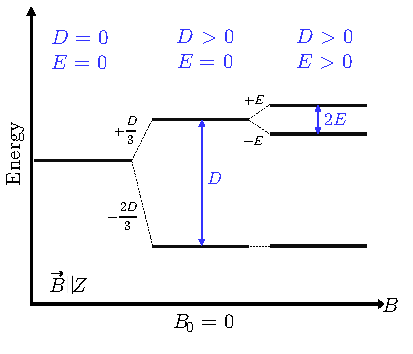
\includegraphics[width=0.6\textwidth]{figures/ZFS.pdf}
    \end{center}
    \caption{Adapted from figure shown in the work by Gr\"{u}ne. }\label{fig:ZFS}
\end{figure}



\subsection{Fine Structure}
The matrix $D$ in \eqref{eq:fine_structure} has form 
\begin{equation}
   D = \begin{pmatrix}
       D_{xx} & D_{xy} & D_{xz} \\ 
       D_{yx} & D_{yy} & D_{yz} \\ 
       D_{zx} & D_{zy} & D_{zz} \\ 
   \end{pmatrix} 
    % \label{eq:}
\end{equation}
which may be simplified by alignment to the wider system axis and diagonalising the matrix as 
\begin{equation}
   D = \begin{pmatrix}
       D_{xx} & 0 & 0 \\ 
       0 & D_{yy} & 0 \\ 
       0 & 0 & D_{zz} \\ 
   \end{pmatrix}.
    \label{eq:fine_splitting_D}
\end{equation}

The \index{trace}{trace} of the matrix $\text{Tr}(D)$ is unchanged by the change of basis. Since for EPR we are only concerned with the changes in energy and not the absolute, we may choose the value of the trace without any loss of generality, so we set it equal to zero. 
\begin{equation}
    \text{Tr}(D) = 0. 
    % \label{eq:}
\end{equation}

This means that the diagonal form of $D$ may be fully determined by just two parameters 
\begin{eqnarray}
    &D &= D_{zz} - (D_{xx}+ D_{yy})/2 \label{fs_D}\\ 
    &E &= (D_{xx} - D_{yy})/2 \label{fs_E}
\end{eqnarray}

Here $D$ represents the axially symmetric parameter and $E$ represents any non-axial contribution of the fine-structure interaction. 

Substituting \eqref{fs_D} and \eqref{fs_E} into \eqref{eq:fine_structure} and expanding allows us to write our fine-structure Hamiltonian as
\begin{equation}
    H_{\ce{FS}} = D \left(\hat{S}_z^2 - \frac{1}{3}S(S+1)\right) + E\left(\hat{S}_x^2 - \hat{S}_y^2\right).
    \label{eq:fine_structure_hamiltonian}
\end{equation}

\subsection{Dipole-Dipole Interaction}
We will now show that the interaction between the magnetic dipoles of two electrons has the same form as \eqref{eq:fine_structure} by considering two electrons ($S=1/2$). 

We begin with the classical expression for the energy between two magnetic dipoles, $\mu_1, \mu_2$
\begin{equation}
    E = \frac{1}{r^3} \left(\mu_1 \cdot \mu_2 -\frac{3(\mu_1 \cdot \vec{r})(\mu_2 \cdot \vec{r})}{r^2}\right).
    % \label{eq:}
\end{equation}

Substituting the quantum mechanical operators for the two electron magnetic dipoles we find 
\begin{equation}
    H_{\ce{DD}} = g_S^2 \mu_B^2 \frac{1}{r^3} \left(\hat{\vec{S}}_1 \cdot \hat{\vec{S}}_2 -\frac{3(\hat{\vec{S}}_1 \cdot \vec{r})(\hat{\vec{S}}_2 \cdot \vec{r})}{r^2}\right).
    % \label{eq:}
\end{equation}

Considering the total spin of the system we may expand this to obtain \cite{carrington1967introduction} 
\begin{equation}
    H_{\ce{DD}} = \frac{1}{2r^5}g_S^2 \mu_B^2 \hat{\vec{S}} \cdot
    \underbrace{
    \begin{pmatrix}
        {r^2 - 3x^2} & -3xy & - 3xz\\ 
        -3xy & r^2 - 3y^2 & -3yz \\ 
        -3xz & -3yz & r^2 - 3z^2 
    \end{pmatrix}
}_{D}
    \cdot \hat{\vec{S}}.
    \label{eq:dd_matrix_form}
\end{equation}

As with \eqref{eq:fine_splitting_D} the matrix $D$ in \eqref{eq:dd_matrix_form} has a constant trace (which we may select to be $0$) leaving the form of the dipole-dipole interaction identical to that of the fine structure interaction 

\begin{equation}
    H_{\ce{DD}} = \hat{\vec{S}} \cdot D \cdot \hat{\vec{S}}.
    % \label{eq:}
\end{equation}

We therefore decompose the traceless matrix $D$ into the axial and non-axial parameters \index{ZFS!$D$}{$D$} and \index{ZFS!$E$}{$E$} as above. 


\subsection{Zero Field Splitting Hamiltonian}
When measuring the values of $D$ and $E$ experimentally, the combined effect will be contained within those measurements so we may therefore describe the zero field splitting interaction as a whole using 
\begin{equation}
    H_{\ce{ZFS}} =D \left(\hat{S}_z^2 - \frac{1}{3}S(S+1)\right) + E\left(\hat{S}_x^2 - \hat{S}_y^2\right).
    \label{eq:ZFS_hamiltonian}
\end{equation}

The effects of $D$ and $E$ on a triplet state are illustrated in Figure~\ref{fig:ZFS}.



% Quardripole? Develop and disregard?
% Nuclear effect - dont even include (or do?)
\section{Nuclear Hamiltonians}

\lipsum[1-4]

% Stark Effect
\section{Stark Effect}
\tdr{Deduce Stark Effect Hamiltonian and write up}
\lipsum[5-8]

%https://journals.aps.org/prl/abstract/10.1103/PhysRevLett.112.087601
\section{Total Hamiltonian}
We now have all the components of our total Hamiltonian for both $S=1$ and $S=3/2$ systems given by
\begin{equation}
   H =  H_{\ce{Zeeman}} + H_{\ce{ZFS}} + H_{\ce{Stark}}
    \label{eq:total_hamiltonian}
\end{equation}
using
\begin{equation}
    H_{\ce{Zeeman}} &= g \mu_B \hat{\vec{S}}\cdot \vec{B}, \tag{\ref{eq:Zeeman_Hamiltonian}}\\ 
\end{equation} 
\begin{equation}
    H_{\ce{ZFS}} &=  D\left(\hat{S}_z^2 - \frac{1}{3}S(S+1)\right)  + E(\hat{S}_x^2 - \hat{S}_y^2),\tag{\ref{eq:ZFS_hamiltonian}}\\ 
\end{equation}

and
\begin{equation}
    H_{\ce{Stark}} &=
                        d_\parallel E_z\left(\hat{S}_z^2 - \frac{1}{3} S(S+1)\right)
                        - d_\perp  E_y(\hat{S}_x^2 - \hat{S}_y^2   ) + d_\perp E_x(\hat{S}_x\hat{S}_y + \hat{S}_y\hat{S}_x).  \tag{\ref{eq:stark_hamiltonian}}
\end{equation}



\section{Spin Hamiltonian}
We can apply \eqref{eq:total_hamiltonian} to our specific $S=1$ or $S=3/2$ system by substitution of the spin operators. They are a matrix representation of the $su(2)$ algebra, equivalent to Pauli matrices in the relevant dimension.
\subsection{$S=1$ Spin Operators}
The three dimensional \index{spin operators!$S=1$}{$S=1$} spin operators $S_j$ in matrix representation are
\begin{equation}
	S_x = \frac{1}{\sqrt{2}} \begin{pmatrix}
		0 & 1 & 0 \\
		1 & 0 & 1 \\
		0 & 1 & 0
	\end{pmatrix},
	S_y = \frac{i}{\sqrt{2}} \begin{pmatrix}
		0 & -1 & 0  \\
		1 & 0  & -1 \\
		0 & 1  & 0
	\end{pmatrix},
	S_z = \frac{1}{\sqrt{2}} \begin{pmatrix}
		1 & 0 & 0  \\
		0 & 0 & 0  \\
		0 & 0 & -1
	\end{pmatrix}.
	\label{eq:s1_spin_operators}
\end{equation}

\subsection{$S=3/2$ Spin Operators}
The four dimensional \index{spin operators!$S=3/2$}{$S=3/2$} spin operators $S_j$ in matrix representation are
\begin{equation}
    \begin{align}
        S_x &= \frac{1}{2} \begin{pmatrix}
            0 & \sqrt{3} & 0 & 0 \\
            \sqrt{3} & 0 & 2 & 0  \\
            0 & 2 & 0 & \sqrt{3} \\ 
            0 & 0 & \sqrt{3} & 0
        \end{pmatrix},&
            S_y &= \frac{1}{{2i}} \begin{pmatrix}
                0 & \sqrt{3} & 0 & 0   \\
                -\sqrt{3} & 0  & 2 & 0 \\
                0 & -2 & 0 & \sqrt{3}\\ 
                0 & 0 & -\sqrt{3} & 0
		\end{pmatrix}, \\
                &
        &S_z = \frac{1}{2} \begin{pmatrix}
            3 & 0 & 0 & 0   \\
            0 & 1 & 0 & 0  \\
            0 & 0 & -1 & 0  \\
            0 & 0 & 0 & -3
		\end{pmatrix}.
        &
    \end{align}
	\label{eq:s1.5_spin_operators}
\end{equation}


\section{Strain and Pressure}
The effect of a strain is treated as an effective electric
field 

% [32] A. E. Hughes and W. A. Runciman, Proceedings of the
% Physical Society 90, 827 (1967).
% [33] G. Davies and M. F. Hamer, Proceedings of the Royal
% Society A: Mathematical, Physical and Engineering Sci-
% ences 348, 285 (1976)


\section{Quantum Sensing}
Quantum sensing involves using a qubit system acting as a quantum sensor that interacts with an external variable of
interest, such as a magnetic field, electric field, strain or acoustic wave, or temperature \cite{Castelletto_2024}. 

Quantum sensors have a higher sensitivity within a nanoscale or microscale sampling volume compared to a fully classical counterpart which would require higher field densities or higher volume interrogation to be effective. 

% Quantum sensing, for example, uses the spin state to acquire a phase shift from interactions with the environment10, and an optical interface (that is, spin-to-photon conversion) allows optical readout of a spin qubit, potentially enhanced by spin-to-charge conversion
\cite{Wolfowicz2021}

% Quantum sensors detect weak physical signals in nanoscale by quantum coherence, quantum properties or quantum entanglement. 
\cite{Kin2021}


% Unlike heritage designs, the magnetometer does not require inductive sensing elements, high frequency radio, and/or optical circuitry and can be made significantly more compact and lightweight,
%....
%Additionally, the robustness of the SiC semiconductor allows for operation in extreme conditions
\cite{Cochrane2016}


% We achieve two-spin interference with a phase sensitivity of 1.79 ± 0.06 dB beyond the SQL and three-spin interference with a phase sensitivity of 2.77 ± 0.10 dB. Besides, a magnetic sensitivity of 0.87 ± 0.09 dB beyond the SQL is achieved by two-spin interference for detecting a real magnetic field. Particularly, the deterministic and joint initialization of NV negative state, NV electron spin, and two nuclear spins is realized at room temperature. The techniques used here are of fundamental importance for quantum sensing and computing, and naturally applicable to other solid-state spin systems.
\cite{Xie2021}

% \paragraph{Qubits}
% A quantum bit or qubit is a simple quantum mechanical system with two eigenstates. 

\subsection{DiVincenzo Criteria}
To construct a working quantum sensor with any candidate system, DiVincenzo and Degen outlined a set of three necessary conditions that must be followed \cite{Crawford2021, RevModPhys.89.035002, DiVincenzo1995}

\begin{enumerate}
    \item The quantum system must have discrete resolvable energy levels (or an ensemble of two-level systems with a lower energy state $\ket{0}$ and an upper energy state $\ket{1}$) that are separated by a finite transition energy. 
    \item It must be possible to initialise the quantum sensor into a well-known state and to read out its state. 
    \item The quantum sensor can be coherently manipulated, typically by time-dependent fields.
\end{enumerate} 

Spin defects are mostly paramagnetic and radiative point defects (or colour centres). Colour centres possessing a 
non-zero electron spin are excellent candidates for optical spin
quantum bits (qubits) \cite{Castelletto_2024}.

Colour centres can produce detectable luminescence even at room temperature. Optical radiation is generally used as a readout but the excitation can also be used for spin manipulation and control.


\cite{RevModPhys.89.035002}
% To construct a working quantum sensor with any candidate material, DiVincenzo[39] and Degen[6] outlined a set of three necessary conditions that must be followed: i) The quantum system must have discrete resolvable energy levels (or an ensemble of two-level systems with a lower energy state |0⟩ and an upper energy state |1⟩) that are separated by a finite transition energy; ii) it must be possible to initialize the quantum sensor into a well-known state and to read out its state; iii) the quantum sensor can be coherently manipulated, typically by time-dependent fields.
\cite{Crawford2021}

\subsection{Crystal Defects}
% Because of about 250 SiC polytypes are known, there should exist more than thousand different spin defects in SiC with distinct characteristics14,15. One can select defects with the most suitable properties for a concrete task, which is not possible for one universal sensor.

\cite{Kraus2014}

% Spin defect centers with long quantum coherence times (T2) are key solid-state platforms for a variety of quantum applications. 
\cite{Kanai2022}

\subsubsection{Quantisation}
\subsubsection{Polarisation}
 % Based on magnetic-dipole forbidden spin transitions, this scheme enables spatially confined spin control, the imaging of GHz-frequency electric fields, and the characterization of defect spin multiplicity
\cite{PhysRevLett.112.087601}

\subsubsection{Coherent Manipulation}
\cite{Widmann2014}

% We find that simultaneous optical reionization and qubit manipulation can be carried out at room temperature with photoexcitation at the typical excitation wavelength used for readout of the divacancy qubits in 4H SiC
\cite{PhysRevB.105.165108}

% These spin defects can be optically addressed and coherently controlled even at room temperature, and their fluorescence spectrum and optically detected magnetic resonance spectra are different from those of any previously discovered defects. Moreover, the generation of these defects can be well controlled by optimizing the annealing temperature after implantation. These defects demonstrate high thermal stability with coherently controlled electron spins, facilitating their application in quantum sensing and masers under harsh conditions.
\cite{Yan2020}


% These defects are optically active near telecommunication wavelengths11, and are found in a host material for which there already exist industrial-scale crystal growth12 and advanced microfabrication techniques13. In addition, they possess desirable spin coherence properties that are comparable to those of the diamond nitrogen–vacancy centre. This makes them promising candidates for various photonic, spintronic and quantum information applications that merge quantum degrees of freedom with classical electronic and optical technologies
\cite{Koehl2011}

% Coherent manipulation of NV centers in SiC has been achieved with Rabi and Ramsey oscillations. 
\cite{Mu2020}


% Hence, coherent control of NV center spins is achieved at room temperature, and the coherence time 𝑇2 can be reached to around 17.1  𝜇⁢s. Furthermore, an investigation of fluorescence properties of single NV centers shows that they are room-temperature photostable single-photon sources at telecom range.
\cite{PhysRevLett.124.223601}

\subsubsection{Efficient Readout}
% Overcoming poor readout is an increasingly urgent challenge for devices based on solid-state spin defects, particularly given their rapid adoption in quantum sensing, quantum information, and tests of fundamental physics. 
% Our results pave a clear path to achieve unity readout fidelity of solid-state spin sensors through increased ensemble size, reduced spin-resonance linewidth, or improved cavity quality factor.

\cite{Eisenach2021}

% we demonstrate the first ever implementation of SCC for VV0 in SiC by performing spin-selective ionization followed by all-optical single-shot readout of the charge state. Using this technique, we can determine an initially prepared spin state with over 80% fidelity. 
\cite{Anderson2022-sf}


% Here, we demonstrate a photo-electrical detection technique for electron spins of silicon vacancy ensembles in the 4H polytype of silicon carbide (SiC). Further, we show coherent spin state control, proving that this electrical readout technique enables detection of coherent spin motion. Our readout works at ambient conditions, while other electrical readout approaches are often limited to low temperatures or high magnetic fields.
\cite{Niethammer2019}


% High-fidelity single-shot spin readout in silicon opens the way to the development of a new generation of quantum computing and spintronic devices, built using the most important material in the semiconductor industry.
\cite{Morello2010}

% Even if the signal-to-noise ratio is reasonably low, a well-trained convolutional neural network (CNN) can predict the resonance peaks of ODMR spectra or the period of Rabi oscillations. Because of the fast output of predictions by the CNN, this method can be used to sense the magnetic field in the environment and microwave intensities in real time.
\cite{PhysRevApplied.17.034046}


\subsection{Coherence}
\cite{Christle2014},\cite{Soltamov2019}, \cite{Gilardoni2020} \cite{BulanceaLindvall2021}, \cite{Astner2022}

% Long coherence times are key to the performance of quantum bits (qubits). 
\cite{Seo2016-ed}

\subsubsection{Spin Relaxation}
\subsubsection{Dephasing}
\subsubsection{Hahn Echo}
% The coherence time of NV defects in the presence of noise originating from parasitic spins located at the diamond interface can be improved by orders of magnitude by using high-order spin echoes.
\cite{Wu2016}
\subsubsection{Example: NV Diamond}


\subsection{Sensitivity}
\cite{RevModPhys.92.015004}

% Our approach is suitable for ensemble as well as single spin-3/2 color centers, allowing for angle-resolved magnetometry on the nanoscale at ambient conditions.
\cite{PhysRevApplied.4.014009}


 % We report the realization of nanotesla shot-noise-limited ensemble magnetometry based on optically detected magnetic resonance with the silicon vacancy in 4⁢𝐻 silicon carbide. By coarsely optimizing the anneal parameters and minimizing power broadening, we achieve a sensitivity of 50nT/√Hz and a theoretical shot-noise-limited sensitivity of 3.5nT/√Hz.
\cite{PhysRevApplied.15.064022}

% By inserting an NV-doped diamond membrane between two ferrite cones in a bowtie configuration, we realize a ∼250-fold increase of the magnetic field amplitude within the diamond. We demonstrate a sensitivity of ∼0.9⁢pTs1/2 to magnetic fields in the frequency range between 10 and 1000Hz. 
\cite{PhysRevResearch.2.023394}


% For all these color centers we saw an enhancement of the photostable fluorescence emission of at least a factor of 6 using micro-photoluminescence systems. Using custom confocal microscopy setups, we characterized the emission of VSi measuring an enhancement by up to a factor of 20, and of NCVSi with an enhancement up to a factor of 7. The experimental results are supported by finite element method simulations. Our study provides the pathway for device design and fabrication with an integrated ultra-bright ensemble of VSi and NCVSi for in vivo imaging and sensing in the infrared.
\cite{Castelletto2019}

 % low photon count rate significantly limits their applications. We strongly enhanced the brightness by 7 times and spin-control strength by 14 times of single divacancy defects in 4H-SiC membranes using a surface plasmon generated by gold film coplanar waveguides.
\cite{Zhou2023}

\begin{group}
\color{lightgray}
Most of the SiC colour centres have a residual spin and
therefore all could be in principle used in quantum sens-
ing. However, they can be distinguished and grouped by their
ground state spin value and the zero field (magnetic) split-
ting (ZFS), which defines their properties and the different
methods for their initialisation, control, and read-out. Colour
centres with the high-spin ground state (S = 1, 3/2) can be
used as two or three levels quantum systems (figure 1(c)). They
can be controlled optically and using a microwave (MW) or
radio frequency (RF) excitation due to the higher sensitivity to
the presence of the magnetic field.


The spin Hamiltonian of an S = 3/2 elec-
tron spin defect within a nuclear spin bath can be written as:

\begin{equation}
    \hat{H} = \underbrace{g \mu_B \hat{\mathbf{S}} \cdot \mathbf{B}_0}_{H_{\text{Zeeman}}} + D \left( \hat{\mathbf{S}}_z^2 - \frac{S(S+1)}{3}\right) + E (\hat{\mathbf{S}}^2_x - \hat{\mathbf{S}}^2_y) + \sum_j \hat{\mathbf{S}}_i \cdot \mathbf{A}_{ij} \cdot \hat{\mathbf{I}}_j
    \label{eq:}
\end{equation}
where g is the isotropic centre specific Lande factor (g =
2.0028), µB is the Bohr magneton, B0 is the external magnetic
field, D and E account for the zero magnetic fields splitting
for the axial (along the spin polarisation axis) or the off-axis
component of the spin defect operator Ŝ = (Sˆx , Sˆy , Ŝz ) respect-
ively. Aij is the hyperfine tensor that describes the central spin
coupling to many nuclear spins indexed by j with spin operat-
ors Iˆj .
\end{group}



\section{Spin Polarisation}\label{spin_polarisation}
\cite{2008}\cite{Weil2006}\cite{Goldfarb2018-he}\cite{Richert2017}
Spin polarisation in the context of EPR is the unequal population of possible spin states. 
For example the differing population of triplet sublevels under the influence of photoexcitation. 
Microwave radiation is only absorbed or emitted in a spin polarised system; so spin polarisation is essential for EPR. 

When the spin is polarised, the unequal population is brought back to equilibrium either by the thermodynamic effect of spin-lattice interactions, or by an induced magnetic resonance transition as is exploited by EPR.

\index{Boltzman statistics}{Boltzman statistics}
% BOLTZMAN STATISTICS

\subsection{Optical Polarisation}
% We find that simultaneous optical reionization and qubit manipulation can be carried out at room temperature with photoexcitation at the typical excitation wavelength used for readout of the divacancy qubits in 4H SiC
\cite{PhysRevB.105.165108}


\section{\index{ODMR}{ODMR}}\label{ODMR}
Optically detected magnetic resonance, specifically continuous wave optically detected magnetic resonance will be the read-out mechanism discussed in this work. This is not necessarily the most sensitive mechanism for any given system, but remains popular due to the very simple implementation. 

The process is to measure the photoluminescence of the spin polarised sample whilst sweeping the driving field to find where the Rabi oscillations occur. When the change of photoluminescence is at a peak, the Rabi frequency is exactly the energy difference between the two spin sub-levels. The energy of and energy difference between the spin sub-levels is dependent on the magnetic and electric field, temperature, pressure and strain. 

\begin{figure}[h]
    \begin{center}
        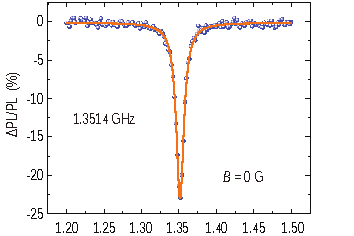
\includegraphics[width=0.5\textwidth]{figures/ODMR.pdf}
    \end{center}
    \caption{
        CW-ODMR spectra for a PL6 defect with $\vec{B} = 0$. Blue dots show data from experiment, the orange line is a Lorentzian fit. Adapted from Li et al.}\label{fig:}
%  CW-ODMR
% spectra in the zero magnetic field. The blue dots are the experimental raw data, and the orange line is the corresponding Lorentzian fitting centred
% at 1.3514 GHz.
    % \cite{Li2021}
    % \todo[inline, color=ediblue]{Write caption}
\end{figure}


Determination of how these physical characteristics influence the change in ODMR spectra is the topic of this work. 


% The results suggest that magnetic field sensing sensitivity can be greatly improved for the optimized laser and microwave power range.
% \cite{PhysRevB.101.064102}


% We measure increased photoluminescence from divacancy ensembles by up to three orders of magnitude using near-ultraviolet excitation, depending on the substrate, and without degrading the electron spin coherence time.
% \cite{Wolfowicz2017}



\section{\index{SiC!Silicon Carbide}{Silicon Carbide}}\label{SiC}

\index{SiC}{SiC} is a semiconductor which can be used for high-power and high temperature electronics \cite{Eddy2009,CASADY19961409}. Many studies have demonstrated SiC's potential as a host material for qubits, which enables the application of SiC quantum sensors even in ambient conditions \cite{PhysRevApplied.6.034001}. Moreover, 
the robustness of SiC allows for operation in extreme conditions
\cite{Cochrane2016}
.

\subsection{Colour Defects in SiC}
Point defects in wide-bandgap semiconductors can have both ground and excited states within the energy gap and, hence, are luminescent centres i.e. colour centres and the luminescence is often stable even at room temperature. 
Many color centers also possess a non-zero electron spin and can be excellent candidates for optical spin qubits \cite{Son2021}.

Multiple colour centres have been observed in SiC, those which may be employed as spin qubits are the divacancy and the Silicon vacancy. 
There are seven types of divacancies in 4H-SiC, the polytype of SiC for which this work will be based. 
The defects can be categorised by their orientation within the lattice. 
These are the c-axis, for which we have the Silicon vacancy V2 and divacancies PL1, PL2, and PL6. 
On the basal axis, we have the divacancies PL3, PL4, PL5, and PL7 \cite{Qin-Yue}. Due to having the highest ODMR contrast 
and coherence at room temperature this work will focus primarily on the c-axis PL6 divacancy and the V2 Silicon vacancy. 
Application of both of these families of defects in quantum sensing can be competitive with the Nitrogen vacancy in diamond \cite{10.1093/nsr/nwab122}.

Figure \ref{fig:SiC_defects} shows the position of the defects in the lattice. 

\begin{figure}[H]
    \begin{center}
        % 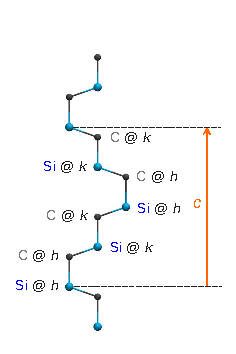
\includegraphics[width=0.32\textwidth]{figures/SiC-non-equiv-sites.pdf}
        % \hspace{1em}
        % 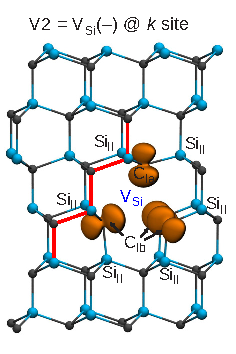
\includegraphics[width=0.32\textwidth]{figures/SiC-V2.pdf}
        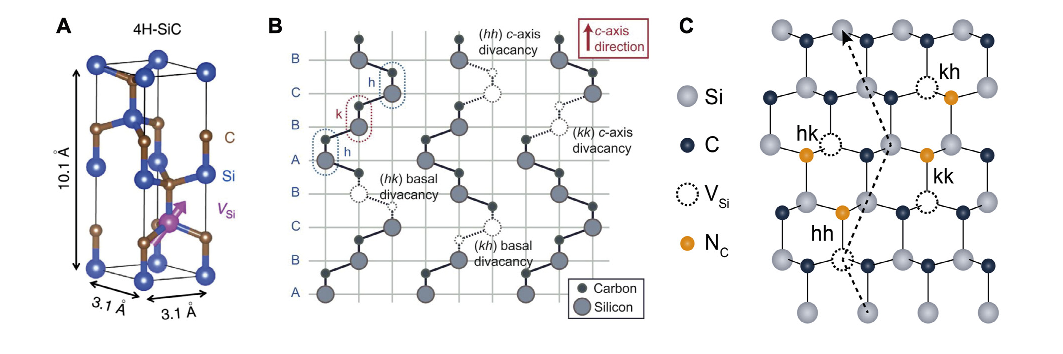
\includegraphics[width=\textwidth]{figures/SiC-lattice.pdf}
    \end{center}
    \caption{(a) Schematic of the 4H-SiC lattice. (b) Possible non-equivalent divacancies sites within the lattice. (c) Schematic of Silicon vacancies within the lattice. Reproduced from Luo et al.}\label{fig:SiC_defects}
    % \cite{Luo2023}
    % \todo[inline, color=ediblue]{Write caption}
\end{figure}



\subsection{Production of SiC}
Whilst the research for the Nitrogen vacancy in diamond is more mature, many equivalent techniques are being developed for 
SiC. 

Diamond is expensive and not compatible with conventional electronic circuits. By comparison, SiC is a technology-friendly material with an existing large-scale production capacity complemented by mature doping techniques \cite{Jiang2023}. Wafer-scale SiC is able to be produced and efficiently manufactured into electronic devices down to the atomic scale \cite{arxiv.1503.07566}.

Divacancies and Silicon vacancies may reliably introduced into SiC. As an example, the Silicon vacancy can be incorporated into the lattice and the density of the vacancies may be controlled down to the single defect level without degradation of the electrical characteristics of the material
\cite{Ohshima2018,PhysRevApplied.4.014009,Wang2019}
.

Further, approaches to manufacture solid-immersion lenses, which may aid the sensitivity or reduce the integration volume of a sensor have been demonstrated
\cite{Sardi2020}
.

Overall, research into the applicability of SiC as a quantum sensor is exciting and shows a lot of potential for application in the near term. 

% we discuss energetic particle irradiation, especially proton beam writing (PBW), in which proton microbeams with MeV range are used, as a method to create VSi in SiC since PBW can create VSi in certain locations with micrometer accuracy and this is very useful to introduce VSi in electronic devices without the degradation of their electrical characteristics.

% Interestingly, VSi can be incorpo-
% rated into SiC nanocrystals [28], and their density can be
% controlled over 8 orders of magnitude down to the single-
% defect level [32].

 % we present the generation and characterization of shallow silicon vacancies in silicon carbide by using different implanted ions and annealing conditions. 

% Here, we demonstrate a scalable approach of manufacturing solid-immersion lenses (SILs) on 4H–SiC.

 
\section{\index{multimodal}{Multimodal Sensing}}
% Using these properties, an integrated magnetic field and temperature sensor can be implemented on the same center.
\cite{Anisimov2016}

 % The effect can be detected as an abrupt reduction of the photoluminescence intensity under optical pumping without application of microwave fields. 
\cite{PhysRevB.100.094104}


% The coherent control of divacancy demonstrates that coherence time decreases as pressure increases. Based on these, the pressure-induced magnetic phase transition of Nd2Fe14B sample at high pressures was detected. These experiments pave the way to use divacancy in quantum technologies such as pressure sensing and magnetic detection at high pressures
\cite{Liu2022}


 % In this paper, we present a self-protected infrared high-sensitivity thermometry based on spin defects in silicon carbide. Based on the conclusion that the Ramsey oscillations of the spin sensor are robust against magnetic noise due to a self-protected mechanism from the intrinsic transverse strain of the defect, we experimentally demonstrate the Ramsey-based thermometry. The self-protected infrared silicon-carbide thermometry may provide a promising platform for high sensitivity and high-spatial-resolution temperature sensing in a practical noisy environment, especially in biological systems and microelectronics systems.
\cite{PhysRevApplied.8.044015}


% Here we show that the defect charge state can also be used to sense the environment, in particular high-frequency (megahertz to gigahertz) electric fields
\cite{Wolfowicz2018}

% we identify the mechanism that polarizes the spin under optical drive, obtain the ordering of its dark doublet states, point out a path for electric field or strain sensing, and find the theoretical value of its ground-state zero-field splitting to be 68 MHz, in good agreement with experiment. Moreover, we present two distinct protocols of a spin-photon interface based on this defect. Our results pave the way toward quantum information and quantum metrology applications with silicon carbide.
\cite{PhysRevB.93.081207}


% We discuss the experimental achievements in magnetometry and thermometry based on the spin state mixing at level anticrossings in an external magnetic field and the underlying microscopic mechanisms. We also discuss spin fluctuations in an ensemble of vacancies caused by interaction with environment.
\cite{Tarasenko2017}

% Moreover, as an example of an application, we demonstrate thermal sensing using the Ramsey method at about 450 K. Our experimental results would be useful for the investigation of high-temperature properties of defect spins and silicon carbide–based broad-temperature-range quantum sensing.
\cite{PhysRevApplied.10.044042}

% The experiments pave the way for the application of silicon carbide-based high-sensitivity thermometers in the semiconductor industry, biology, and materials sciences.
\cite{D3NR00430A}


% The experiment implies the feasibility of using implanted NV centers in high-quality diamonds to detect temperatures in biology, chemistry, materials science, and microelectronic systems with high sensitivity and nanoscale resolution.
\cite{PhysRevB.91.155404}

% . We then use it to detect the strength of an external magnetic field. Finally, we use the Ramsey methods to realize a temperature sensing with a sensitivity of 163.2 mK/Hz1/2. The experiments demonstrate that the compact fiber-coupled divacancy quantum sensor can be used for multiple practical quantum sensing.
\cite{Quan:23}

% These results establish SiC color centers as compelling systems for sensing nanoscale electric and strain fields.
\cite{PhysRevLett.112.087601}




% Consider Including
% \section{To Sort (abstracted)}
% \input{Sections/HahnEcho.tex}
% \input{Sections/SpinBaths.tex}
% \input{Sections/SpinCoupling.tex}
% \section{Defect Orientation}

Colour centres or defects in general are part of the crystal lattice and thus have an associated orientation and direction within the lattice. This allows the definition of a \textbf{defect axis}. For example, in diamond the NV axis is defined as the vector from the vacancy towards the Nitrogen atom when the vacancy is taken as the origin of your co-ordinate system. 

In a tetragonal crystal, due to symmetry there are four possible orientations of a defect within the lattice: $111$, $1\overline{11}$, $\overline{1}1\overline{1}$ and $\overline{11}1$ directions. 

\section{Miller Indices}
The notation for defect orientation above is known as a Miller Index, and we consider the $111$ direction to be aligned with the defect axis. 

This means that if we know the orientation of our crystal then we can establish the orientations of the defect axis inside. For example, using a crystal for which all surfaces belong to the $\{001\}$ lattice planes, each surface normal is aligned with a Cartesian axis. Thus, by fixing the crystal in place, there remain just \textbf{four} possible angles which a defect axis can have with respect to the crystal surface.

Calculating the scalar product of any of the surface planar directions in the family of $\{001\}$ and the four possible orientations of the defect within the lattice we find $\cos\theta = \pm0.6$. Then, considering the physical solutions (from $0, 2\pi$) gives four possible angles that the (directed) defect axis may make with the surface of the crystal: $53.13^\circ$, $306.87^\circ$, $126.9^\circ$ and $233.13^\circ$ ($0.927$, $5.355$, $2.214$ and $4.069$ radians respectively). 






    


% \input{Sections/SpinDetection.tex}
% \input{Sections/SpinRelaxation.tex}
% \input{Sections/DensityMatrices.tex}
% \input{Sections/RabiOscillations.tex}
% \input{Sections/SpinInitialisation.tex}
% \section{Lattice Symmetry}
Tetragonal lattice has the $$

% \input{Sections/StokesShift.tex}
% \section{Linear Combination of Atomic Orbitals}


